\documentclass[sigconf, screen, nonacm]{acmart}

\usepackage{multirow}
\usepackage{tabularx}
\usepackage{caption}
\usepackage{subcaption}

%%
%% end of the preamble, start of the body of the document source.
\begin{document}

\title{Object Instance Segmentation for Better Distinguishability in In-Door Scenes}

%%
%% The "author" cmman and its associated commands are used to define
%% the authors and their affiliations.
%% Of note is the shared affiliation of the first two authors, and the
%% "authornote" and "authornotemark" commands
%% used to denote shared contribution to the research.
\author{Roman Beltiukov}
\authornote{All authors contributed equally to this research.}
\email{rbeltiukov@ucsb.edu}
\orcid{0000-0001-8270-0219}
\affiliation{%
	\institution{University of California, Santa Barbara}
  \city{Santa Barbara}
	\state{CA}
	\country{USA}
}

\author{Liubov Kurafeeva}
\email{liubov\_kurafeeva@ucsb.edu}
\authornotemark[1]
\affiliation{%
	\institution{University of California, Santa Barbara}
  \city{Santa Barbara}
	\state{CA}
	\country{USA}
}


\author{Francie Wei}
\authornotemark[1]
\email{hwei@ucsb.edu}
\affiliation{%
	\institution{University of California, Santa Barbara}
  \city{Santa Barbara}
	\state{CA}
	\country{USA}
}


%%
%% The abstract is a short summary of the work to be presented in the
%% article.
\begin{abstract}
A clear and well-documented \LaTeX\ document is presented as an article
formatted for publication by ACM in a conference proceedings or journal
publication. Based on the ``acmart'' document class, this article presents 
and explains many of the common variations, as well
as many of the formatting elements an author may use in the
preparation of the documentation of their work.
\end{abstract}


%%
%% Keywords. The author(s) should pick words that accurately describe
%% the work being presented. Separate the keywords with commas.
\keywords{bionic vision, objects identification, indoor scenes}



\begin{teaserfigure}
	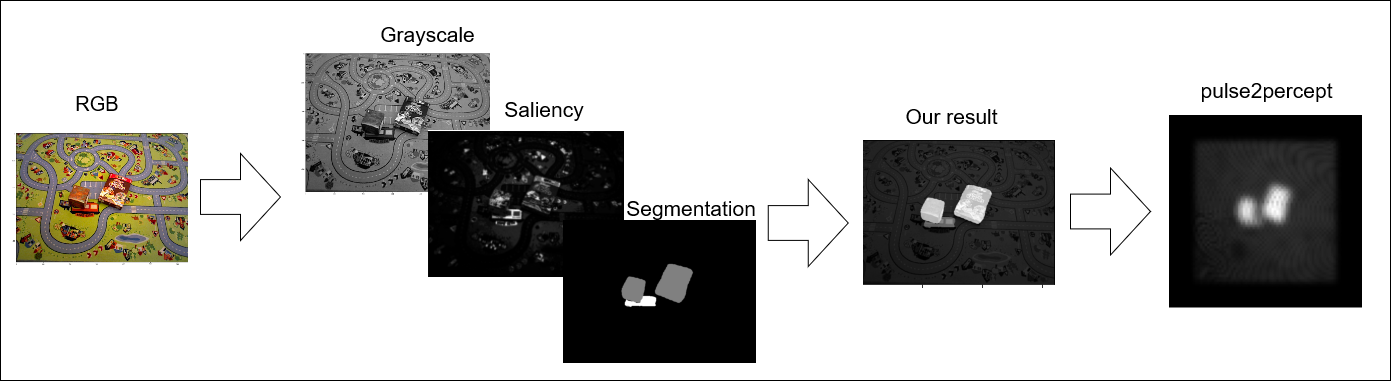
\includegraphics[width=\textwidth]{figures/teaser.png}
	\caption{Proposed method of combining recolored segmentation results, saliency map and background to highlight objects and allow to better distinguish them.}
\end{teaserfigure}

%%
%% This command processes the author and affiliation and title
%% information and builds the first part of the formatted document.
\maketitle

% Intro section
\section{Introduction}
ACM's consolidated article template, introduced in 2017, provides a
consistent \LaTeX\ style for use across ACM publications, and
incorporates accessibility and metadata-extraction functionality
necessary for future Digital Library endeavors. Numerous ACM and
SIG-specific \LaTeX\ templates have been examined, and their unique
features incorporated into this single new template.

If you are new to publishing with ACM, this document is a valuable
guide to the process of preparing your work for publication. If you
have published with ACM before, this document provides insight and
instruction into more recent changes to the article template.

The ``\verb|acmart|'' document class can be used to prepare articles
for any ACM publication --- conference or journal, and for any stage
of publication, from review to final ``camera-ready'' copy, to the
author's own version, with {\itshape very} few changes to the source.

% Related work
\section{Related work}
Most retinal bionic vision implants utilize a stream from an external video camera and provide preprocessed images to the user. Being physically rather close to natural human sight, we can apply standard techniques of image preprocessing like rescaling, edge detection, Gaussian blur, and others. Several works \cite{AYTON20201383, humayun2009preliminary} that study bionic implant users states that increasing the contrast of objects and providing them simplified scenes increases their orientation skills and allows them to complete tasks more efficiently. 

With new implants being developed, scientists suppose increasing of the computational power of Video Processing Units so it possibly can hold additional tasks connected with more complex image preprocessing methods, starting with seam carving \cite{AlAtabany2010} and up to introducing semantic segmentation of the whole image \cite{HORNE2016113}. 

Most of the recent papers which tried to enhance bionic vision tried to apply different saliency detection algorithms and add this information to the image \cite{LI20171, LI201864, Parikh_2010, 6091267, aor12498}. Saliency information is defined as information about image pixels that differ from surroundings, so the human eye would typically focus on them. To obtain a saliency map, there exist deep learning models \cite{kmmerer2016deepgaze} that provide qualitative predictions. However, despite saliency maps being useful, they are \textit{purpose-agnostic} so they highlight the information no matter what the task is and therefore wouldn't help much to search certain objects. 

Several papers also introduced using depth information \cite{Perez-Yus_2017_ICCV, McCarthy_2014} to enhance the image and provide the user some additional context. Unfortunately, these papers focused on an outdoor environment where depth sensors indisputably would help locate dangerous objects. Still, very little information about indoor objects search and any tasks except the basic location are presented.

The idea of applying segmentation or object detection models to the video stream isn't new in this area, as several papers have tried to do this. The paper by Weiland et al. \cite{6345928} tried to adjust the object detection algorithm to facilitate objects' location on the empty white table. However, objects were pretty separated and located far from each other. The paper by Horne et al. \cite{HORNE2016113} also introduced semantic segmentation of the image, but they tried to segment all the images and highlight those areas which are important in terms of outdoor navigation. Besides that, in the recent work of Han et al. \cite{han2021deep} a rather close approach was presented but with a focus on the outdoor environment. 

Finally, the closest to our ideas Sanchez-Garcia et al. \cite{visapp19} work was published two years ago. This paper introduces fully convolutional networks to segment the objects in indoor scenes. Despite being very close to our work, the paper focuses on directly highlighting the objects considering they are already far from each other and do not involve the separation task of adjacent objects. The authors directly assign a constant brightness level to every object and do not scrutinize situations when objects are in front of each other or located very close. To further separate our work from this paper, we focus on small objects and everyday items that bionic implant users possibly want to find and locate inside the room or other indoor location.

% Methods
\section{Methods}
\label{methods:general}

To provide better visual objects separation, we focus on adding visual highlighting information to the original picture
changing original brightness of the objects. Initially (see \autoref{methods:processing}), we convert the original image to grayscale, then we use the saliency model to obtain saliency map information. After that, we run an instance segmentation model on the same original image to get instance segmentation masks of the predefined allowed list of classes). Given the masks, we construct a graph on a base of these masks where objects are vertices, and each edge corresponds to two objects being adjacent to each other. After creating the graph, we apply the graph coloring strategy to assign brightness to these objects and recolor them to separate the objects better (in the \autoref{methods:recoloring}). Given all these layers (saliency map, grayscale image, and colored segmentation results) in \autoref{methods:combining} we combine them together to produce the final result to be provided to the user. Finally, in {\autoref{methods:survey}} to evaluate the results, we processed our images with the pulse2percept model and conducted a user study in order to measure the improvement.

\subsection{Dataset}
\label{methods:dataset}

We chose Object Clutter Indoor Dataset \cite{ociddataset} to use as visual stimuli for our research.
This dataset provides 96 different cluttered indoor scenes with different objects that you can find in the room. 
Each scene is located on either floor or the table and represents a typical scenario where the bionic implant user needs to find an object in a pile of similar objects or near some background. We chose a subset of pictures from the dataset to reduce calculations but tried to keep different backgrounds to make the research more representative.
For each picture from the dataset, there exist RGB picture, point cloud, depth map, and label information, but we kept only RGB to represent the most popular RGB video cameras suited for implants.

\subsection{Processing the image}
\label{methods:processing}

As we design our solution for daily indoor scenarios, we need to keep original picture information and provide it to the user.
Considering the current restrictions of bionic vision implants, we convert the image to grayscale using standard conversion weights. In addition to it, we extract saliency map information from the original color image using the DeepGaze II model \cite{kmmerer2016deepgaze}. Saliency models predict how people look in images and provide valuable feedback on what places to highlight, as this would be interesting to pay attention to. Given that the original background would be dimmer than before, we believe it is important to highlight important places and structures besides the objects as this information can be critical. 

In parallel to saliency reconstruction, we invoke a segmentation algorithm on the original color image. We use detectron2 model \cite{wu2019detectron2} with pretrained weights on LVIS dataset \cite{gupta2019lvis} named 'X101-FPN' in the detectron2 Model Zoo. The LVIS dataset is a dataset for large vocabulary instance segmentation that incorporates more than 1200 categories of objects, including typical indoor objects like fruits, pens, and others. This dataset is, to our knowledge, the best-suited dataset for indoor instance object segmentation with pre-trained models available in detectron2 Model Zoo. After segmentation, we filter the results and keep only masks of classes from the predefined allowed list of classes where we enlisted the most popular indoor objects categories available in the LVIS dataset. This list intentionally does not contain several classes (like table, carpet, and others) as these objects are usually not the target to be found by bionic vision users. In addition to filtering the classes, we also remove objects whose size is less than certain hyperparameters. Besides that, we also look for pair of objects which intersect heavily and remove one of them. We calculate Intersection-Over-Union (IoU) metrics for that.

After segmentation masks are obtained, we construct a graph from these masks. As segmentation only provides us a list of objects to highlight, we need to properly assign them different brightness to make them easily visually separable from each other. To achieve this, we create an adjacency graph of these objects where each node corresponds to an object, and if two objects are close to each other on the image (so the distance between their closest points is less than the corresponding hyperparameter), then the edge between these objects is created. This graph later is subject to the graph coloring algorithm. This algorithm tries to assign different colors to adjacent nodes, which greatly fits our strategy of highlighting the adjacent objects differently to make them different. We use standard greedy algorithm \cite{kubale2004graph} with largest\_first strategy. After coloring is finished, the adjacent objects are assigned different color classes, and the whole graph (and therefore the whole image) uses the least possible amount of colors. As for the grayscale image only changes in brightness are available, reducing the overall amount of classes increases the brightness difference between the classes and makes objects of different color classes more distinguishable.

\subsection{Recoloring}
\label{methods:recoloring}

The main disadvantage of the graph coloring algorithm is a lack of ordering in coloring. For example, given object A with color class 1, for the coloring algorithm there is no difference in assigning classes 2 or 3 to the adjacent objects. However, as we want adjacent objects to be not only different but most possibly different, we want to assign the most different brightness values to adjacent objects. To achieve this, we use recoloring strategy on top of the resulting colored graph.

The primary purpose of recoloring strategy is to make static mapping between current color classes assigned to each node to new color classes where the difference between adjacent objects increases. This mapping is global for the whole graph, so if the strategy decides to change color class 1 to color class 5, this change would be applied to all color class 1 objects (so they become of color class 5), and no more color classes would be mapped to color class 5. As we plan to directly transform color classes to corresponding brightness levels, we value the situation where objects of color classes 1 and 5 are adjacent greater than where the same objects are of color classes 1 and 2. To reassign the labels, we created several different recoloring strategies.

The currently used recoloring strategy is based on top of the breadth-first search algorithm. It starts with a random node, assigns the biggest class to this node, and takes all neighbors whose classes are not reassigned yet. Next, all these neighbors classes are reassigned, so they differ the most from the current node and each other, and then the algorithm deletes assigned color classes from the list of available color classes and recursively starts from these nodes, and works until all classes are remapped.

We noticed that this algorithm, on average, produces better coloring results than the default coloring greedy strategy and other recoloring algorithms, but this statement is yet to be proved via user survey in future work.

After recoloring the graph, we provide these labels to the objects and transfer them to the single two-dimensional layer to be used later in combination with other layers.

\subsection{Combining the results}
\label{methods:combining}

The resulting segmentation map is being rescaled to the $[0.255]$ range to be treated as a valid greyscale image. This map alone theoretically could be passed to bionic implant users, but it would pose a risk of hiding the objects not being recognized but still crucial for the user.

To provide background information for the segmented objects, we would like to add more information on the recolored segmentation maps. Therefore, we tried several mixing methods and concluded that combining grayscale maps and recolored segmentation maps would bring the best result.

We first tried to combine the saliency map and the recolored segmentation map by modifying the method given in the previous paper \cite{han2021deep}, as the saliency maps can include the region of interest in the background. We first thresholded the saliency map to only retain 30\% of the most salient region and then added them to the place where nothing is segmented in the recolored segmentation map. However, the combined map only adds small undistinguishable artifacts on the recolored segmentation map. When we transform it into simulated prosthetic images, it does not introduce significant changes to the simulated prosthetic images transformed from the recolored segmentation map.

We then tried to combine the grayscale map and the recolored segmentation map. The grayscale map would be x\% percent of the combined image, and the recolored segmentation map would be (100-x\%) percent of the image. We tried many x values and suggested that 30 would be the best value to include information in the grayscale map differentiated from the recolored segmentations.
To make the grayscale map much clearer in low percentage in the combined map, we tried increasing the contrast of the grayscale maps or thresholding the grayscale map into binary. However, they both introduce significant changes in the shape of the background objects (like tables) that make the background hard to understand both the combined map and in simulated prosthetic vision images.

\subsection{User study}
\label{methods:survey}

To estimate the changes, we considered surveying objects' distinguishability on images as bionic implant users see them. 
The processed images from previous steps were then transformed into simulated prosthetic images using open-source library pulse2percept \cite{Beyeler148015}. The images would be the input stimuli to the pulse2percept simulator. The simulator downscaled the processed images into the electrode array size and assigned each pixel in the processed image to an electrode. The grayscale value of the pixel determines the current on the electrodes. The size of the electrode array in our simulation is 32x32, which is a possible size of an electrode array in current or developing retinal implants, and shows good performance on identifying people and cars in the outdoors scene in the previous paper \cite{han2021deep}.

We used the axon map model in the pulse2percept library. The shape of the phosphene in the model is determined by parameters rho and axlambda, where rho is the exponential decay constant away from the axon and axlambda is the exponential decay constant along the axon. Since the actual phosphene shape varies among patients, we tried several possible pair of rho and axlambda and chose the one (rho = 70, axlambda = 30) that show the difference in coloring.

We created a subset of 15 randomly chosen images and applied our algorithm to produce versions of them with highlighted objects. Then we processed each image with the chosen pulse2percept model to represent a typical perception of these images by a bionic implant user. We then created a publicly available website where we asked people to estimate the number of objects on the given picture. We neither stated whether this picture was original or preprocessed nor described the research idea to the subjects. 

% Results
\section{Results}
Lorem ipsum dolor sit amet, consectetur adipiscing elit. Curabitur pretium, neque efficitur ultricies feugiat, quam turpis efficitur nisi, nec tempus lacus felis hendrerit est. Duis pretium interdum enim, non lobortis magna malesuada lacinia. Pellentesque habitant morbi tristique senectus et netus et malesuada fames ac turpis egestas. Morbi at ultricies felis, blandit porttitor odio. Nunc at lacus condimentum, gravida odio bibendum, mollis ex. Donec in ex augue. Quisque tellus nunc, pretium sit amet eleifend id, condimentum eget neque. Nulla mattis fermentum pellentesque. Proin sodales sem ex. Aliquam non leo id lorem luctus consectetur. Nulla molestie, mauris sed hendrerit aliquet, mi nisi rhoncus ipsum, non mollis lacus nulla vehicula ante. Sed neque dolor, porta vitae magna vel, pretium accumsan urna. Proin sit amet ante ut enim viverra finibus. Aenean aliquam venenatis sapien et imperdiet. Donec tempor auctor ante.

Integer dolor urna, pharetra id nunc at, mollis dignissim nulla. Sed tincidunt dui at tortor vulputate, vitae mattis tortor maximus. Praesent euismod dui enim, nec blandit libero molestie et. Nulla vitae mauris hendrerit, posuere quam elementum, feugiat leo. Cras sit amet purus at mi consectetur luctus. Cras venenatis felis ac purus luctus ultricies. Nunc in euismod eros. Sed urna ligula, egestas fermentum efficitur a, gravida in tortor. Phasellus volutpat suscipit pulvinar.

Etiam pharetra, lacus id hendrerit hendrerit, ligula dui luctus ex, ut fermentum sem justo nec purus. Donec eu elit sed dolor porta luctus non vitae urna. Aliquam sollicitudin lacus id eros consectetur, quis hendrerit orci vulputate. Sed placerat tempor risus eget venenatis. Vivamus ac sagittis lacus, eu egestas leo. Nunc pellentesque vehicula commodo. Fusce quis mauris nisl. Nullam sed augue maximus arcu semper lacinia. Maecenas mattis erat ante, non suscipit metus finibus a. 

% Discussion
\section{Discussion}

In this work, we combined different deep-learning models and graph theory to process pictures to facilitate objects finding, separation, and estimation for bionic implant users. We simulated bionic implant vision via open-source implementation of computational models of bionic vision, compared original pictures with their modified versions, and proved that our findings at worst do not complicate solving the tasks stated above but often facilitate it and improve human efficiency. We also made all the code and results available on \url{https://github.com/maybe-hello-world/team_blue_291A}.

\subsection{Possible improvements}

Despite being visually attractive, the results do not always introduce a significant change to the user's ability to solve the task. We want to mention two different possible problems to overcome to make the difference more noticeable:
\begin{enumerate}
    \item Segmentation model threshold attenuation. Several hyperparameters (like threshold and non-max suppression) need to be modified during the inference of the network. We found this step especially complicated during the research due to the lack of computing resources for that. Still, given the needed amount of time, the segmentation network could be adjusted to reduce the number of false-positive objects. For example, we had to exclude some classes from the segmentation process (like the `toy` class) because they provided too many false positive masks. We believe that reducing the number of the model's errors would increase the solution's overall performance.
    \item Development of new recoloring strategies. For the paper, we implemented a relatively simple BFS-related recoloring strategy which does not always produce positive results according to our observations. We suggest providing a better recoloring approach would help to highlight the objects more qualitatively and facilitate their visual separation further. 
\end{enumerate}

\subsection{Dataset for estimation}
For the initial iteration of the research, we took the dataset with different objects stacked together to emphasize the possibility to visually differ them and estimate their total amount. To better demonstrate the method, we suggest testing this solution in the clumsy environment with different obstacles provided and objects not in the center of the frame. Initial LVIS dataset could be a good starting point for future work, though trying to spread the research on video stream estimation could require custom dataset collection. 

\subsection{Survey}
Due to limited time and people to survey, we couldn't score all coloring and mixing strategies and collect feedback on a broader set of pictures. In the future, we suggest spending more time and resources on it to find the best possible strategy, better measure performance, and find situations where our solution works better. 

\subsection{Future work}
For future work based on this research, we suggest overcoming the mentioned problems of our work and enhancing it to the degree of providing helpful assistance to bionic vision implant users. Stabilizing of segmentation and recoloring process together with network distillation to lower resource consumption would provide a better experience and can advance this research to the point of applicability for real devices. In addition to that, we see a potentially exciting improvement in implementing the audio interface for the segmentation network that would allow changing allowed classes for segmentation on the fly. That would provide an interesting experience of a user being able to highlight only needed objects and provide them theoretically better-than-human visual perception in certain situations. 

%
%% The next two lines define the bibliography style to be used, and
%% the bibliography file.
\bibliographystyle{ACM-Reference-Format}
\bibliography{references}

%%
%% If your work has an appendix, this is the place to put it.
\appendix

\section{Additional materials: Survey histograms}

\begin{figure*}[h!]
    \label{survey:separate}
    \centering
    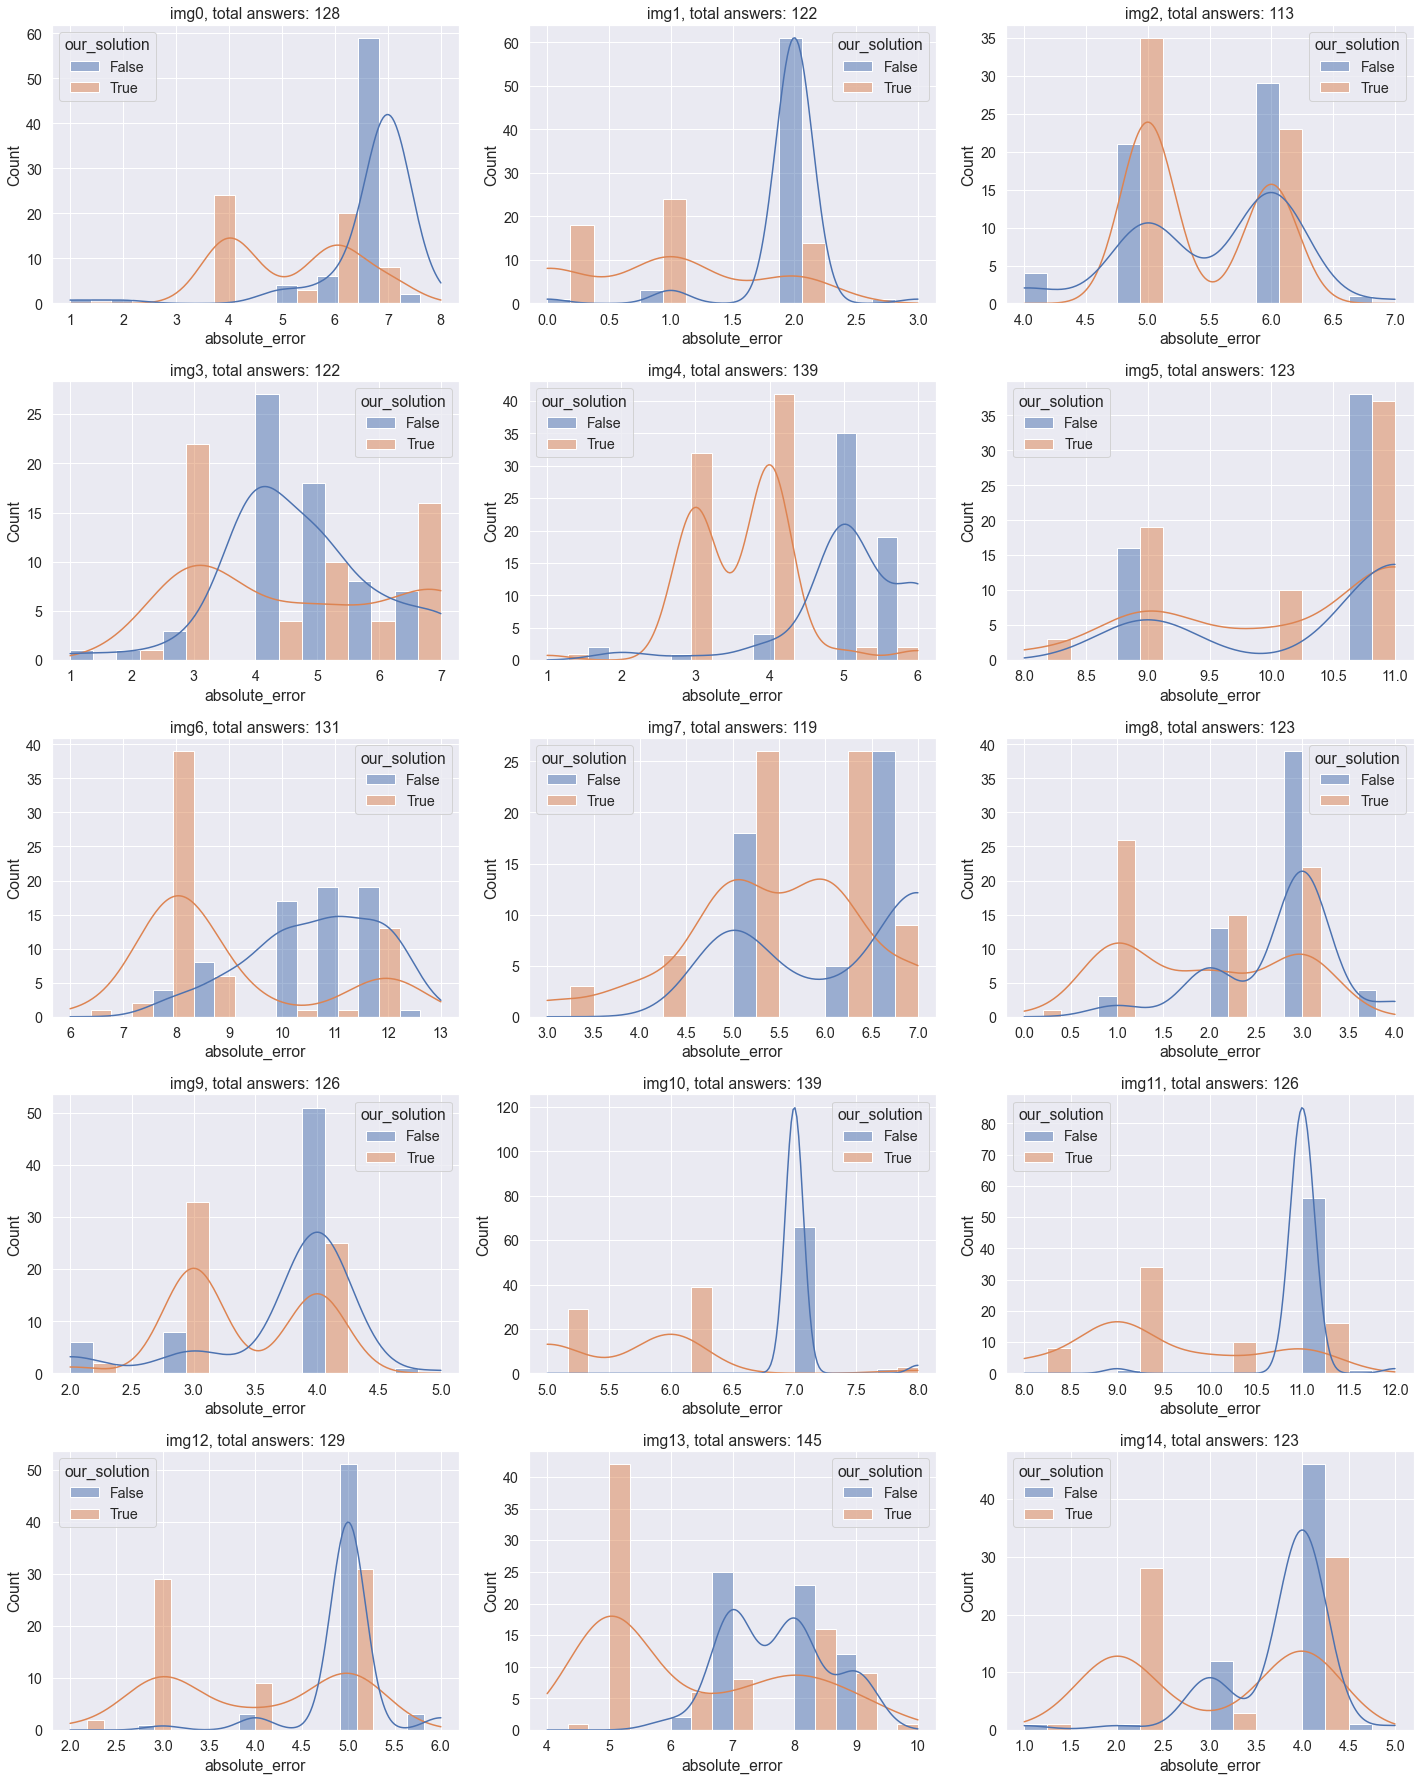
\includegraphics[width=\linewidth]{figures/survey_separate.png}
    \caption{Histograms of errors for each picture from the test dataset}
    \Description{Distributions of modified images are constantly better then original.}
\end{figure*}
\begin{figure*}[h!]
    \centering
    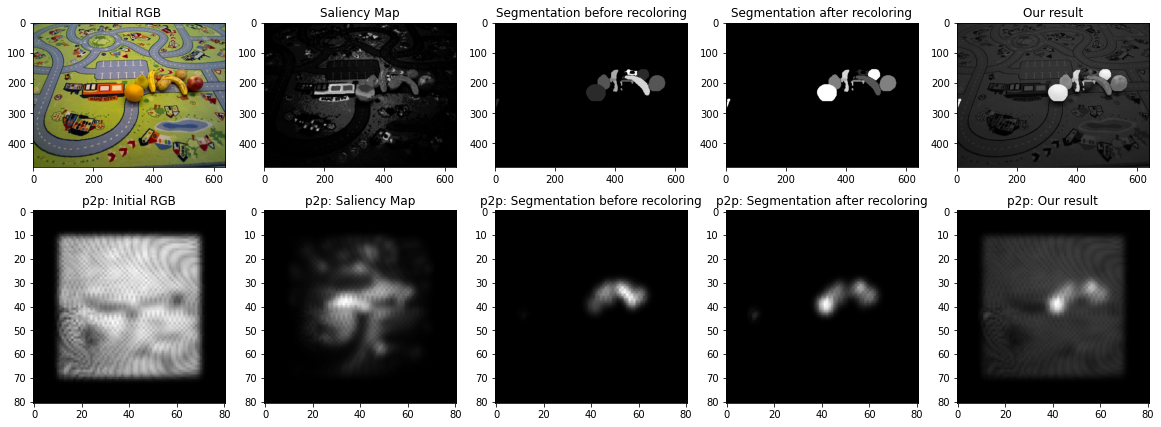
\includegraphics[width=0.8\linewidth]{figures/appendix1.png}
    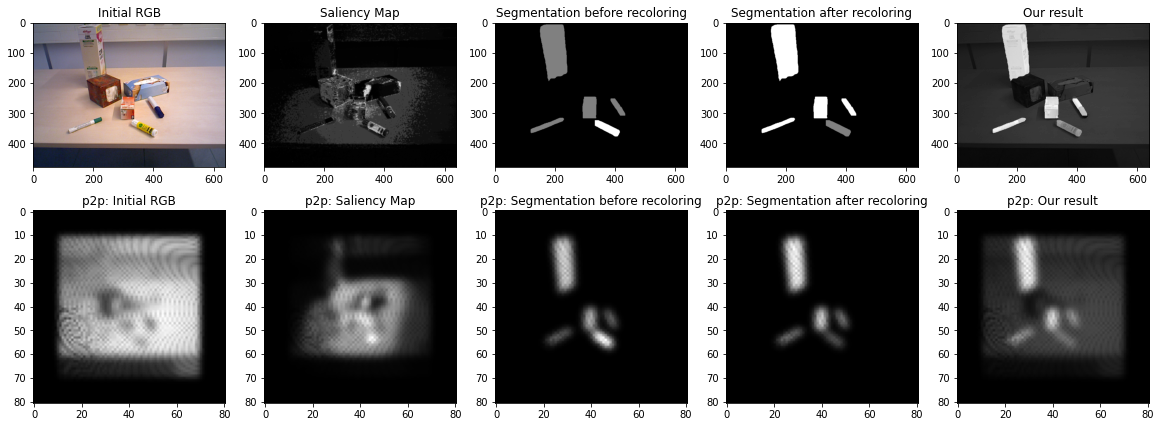
\includegraphics[width=0.8\linewidth]{figures/appendix2.png}
    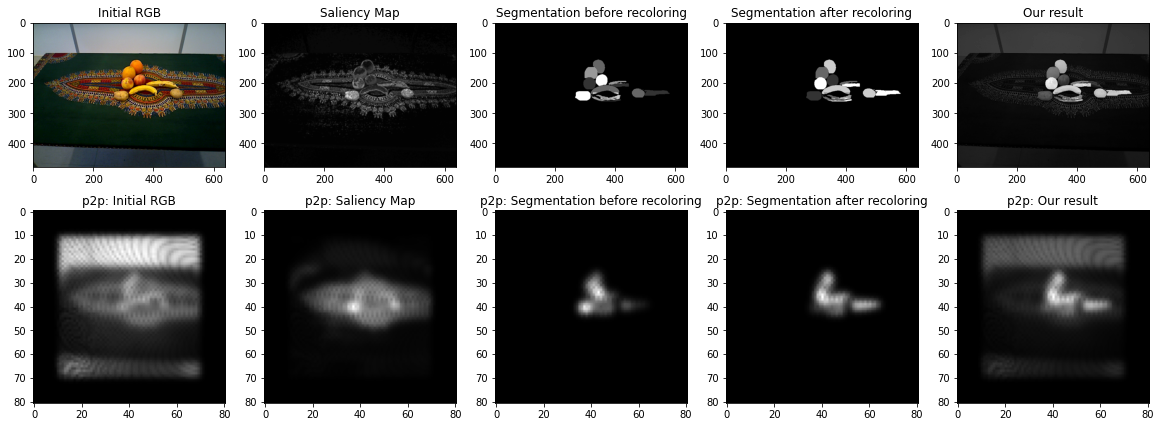
\includegraphics[width=0.8\linewidth]{figures/appendix3.png}
    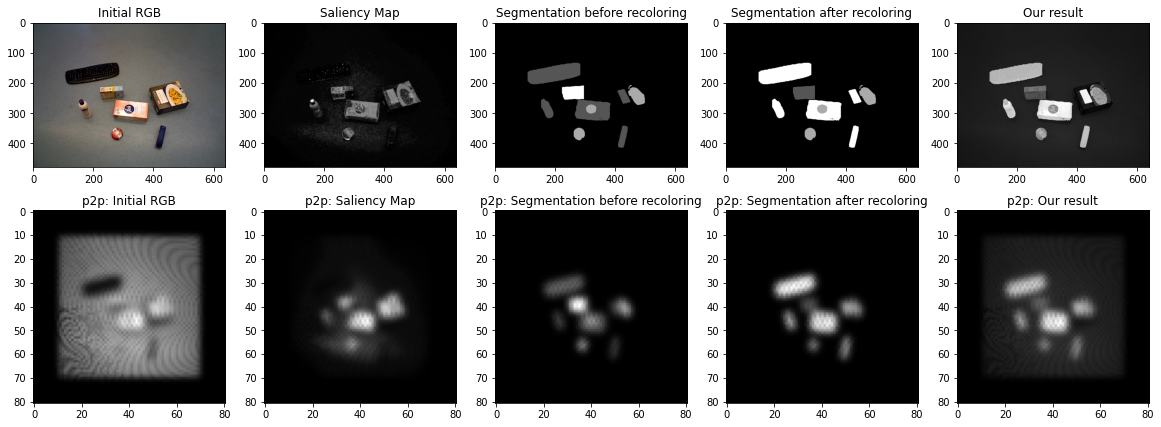
\includegraphics[width=0.8\linewidth]{figures/appendix4.png}
    \caption{More examples of picture processing showing an improvement in objects detection.}
    \label{appendices:processing}
\end{figure*}

\end{document}
\endinput
%%
%% End of file `sample-sigconf.tex'.
